\chapter{Methodology}

\section{Salinity Measurement Method}
A \gls{ctd} sensor, which measures salinity using conductivity, temperature and depth, was chosen as the salinity measurement device.
When choosing a measurement technique multiple factors needed to be considered.
Firstly, the salinity measurements are to be conducted in the Antarctic, where the environment, and remote nature of the area, make majority of the measurement methods unusable.
Secondly, the device would need to fit through an ice core hole with a diameter of $100mm$, and lastly, the device would need to be able to take continuous measurements.

\gls{ctd} sensors do not require sample collection, unlike chlorinity titration, gravimetric analysis and refractometry.
This removes both the need for sample collection and the challenges of sample degradation, storage and transport logistics.

Modern \gls{ctd} sensors are compact, and can easily be designed for specific space constraints.
This coupled with its deployments flexibility make it the preferred choice over methods, such as laboratory methods, which suffer from deployment constraints.
\gls{ctd} sensors allow for continuous realtime monitoring, a characteristic none of the the alternative methods provide.
The alternative methods either require sample collection, or cannot measure continuously.

\gls{ctd} instruments inherently measure conductivity, temperature and pressure simultaneously, providing salinity measurements with temperature and depth compensation, whereas laboratory methods measure salinity only, and require separate temperature measurements.


These factors coupled with the researcher's significant experience with PCB design and electronics influenced the choice for a \gls{ctd} sensor.

\section{Electrode Design}\label{sec:electrode_design}
When measuring conductivity, choosing an electrode material plays a significant role in the accuracy of the measurements.
To get an accurate measurement of the resistance of the water, ideally, a electrode resistance of zero is required.
This would allow the resistance measurement to be entirely due to the resistance of the water.
Most conductive materials have conductivities of order $10^6 - 10^8 S/m$, which is negligible compared to sea (salt) water, which has an average conductivity of $3.31 S/m$~\cite{conductivities}\cite{ocean_conductivity_tyler}.
Preferably, the material with the highest conductivity, silver, would be used. However, conductivity is not the only factor considered when designing an electrode. 
The electrodes will be submerged in saltwater, which is highly corrosive. The material chosen will require high corrosive resistance. 
Silver, though having the highest conductivity, has a low corrosion resistance, and therefore cannot be used in this application~\cite{zhang_silver}.

Titanium is the material of choice for ocean-use~\cite{materials_ocean_structures}. It is essentially corrosion-free, and offers a conductivity of $2.68\times 10^{6}$~\cite{conductivities}.
However, titanium is expensive and fell out of the budget of this project.
Gold boasts both a high conductivity of $4.10\times 10^{7}$, higher than titanium but lower than silver, and a high corrosion resistance, making it an ideal choice.
Gold is also a commonly used material in electronic design, with it being used in \gls{pcb} manufacturing, to protect copper pads from corrosion.
This is done through a \gls{enig} plating process, where a layer of nickel is chemically deposited onto the exposed copper traces, to prevent the copper from oxidizing, and then a layer of gold is applied over the nickel through an emmersion process, to protect the nickel.
This process is significantly more expensive compared to standard \gls{pcb} manufacturing, however, it allowed for the use of gold electrodes, and therefore was factored into the budget. 

In order to utilise the \gls{enig} process a \gls{pcb} was used to design the gold electrodes.
This allowed the electrodes to be designed with a known area and separation distance, allowing for accurate conductivity calculations.
A solder pad was used to design the portion of the \gls{pcb} that would act as the electrode, since it allowed the copper/gold to be exposed.
Then during manufacturing \gls{enig} was chosen as the surface finish, to achieve the gold finish.

The \gls{pcb} was designed to allow for easy calculation of the conductivity $\sigma$, using the equation below:
\begin{equation}\label{eqn:conductivity}
    \sigma = \frac{L}{RA}
\end{equation}

where $L$ is the distance between the electrodes, $R$ is the resistance of the water, and A is the cross-sectional area of the electrodes.
A square face of $20mm\times 20mm$ was chosen to allow for easy cross-sectional area calculations, and a distance of $10mm$ was chosen as the separation distance.
This distance was chosen as it is close enough to reduce current spreading, but not too small to where the water could not flow easily between the electrodes.
A $2mm$ fringe guard was added around the main electrode area to reduce current fringing, which is an effect that causes the current to spread beyond the edges of the gap~\cite{roshen_fringing}.
The fringe guards counteract this by saturating the area surrounding the main pads with current, preventing them from fringing.

The resistance of the electrodes was calculated using the Equation~\ref{eqn:conductivity} and was found to have an approximate resistance of $7.55\Omega$

The electrode \gls{pcb} was designed with the consideration of mounting to the probe \gls{pcb}.
To accommodate this, solder pads were added to allow the electrodes to be soldered to the probe \gls{pcb}.
Mounting legs were also factored into the design to ensure that the electrodes stayed straight and secure.
The design can be seen in Figure~\ref{fig:electrode_pcb}.

\begin{figure}[H]
    \begin{minipage}{0.5\textwidth}
        \centering
        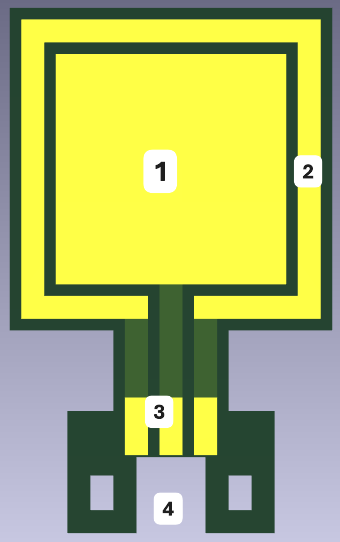
\includegraphics[width=0.6\textwidth]{Figures/electrode_pcb.png}
    \end{minipage}
    \begin{minipage}{0.5\textwidth}
        \centering
        \begin{tabular}{cl} \hline
            1 & Main Pad \\ \hline
            2 & Fringe Guard \\ \hline
            3 & Solder Pads \\ \hline
            4 & Mounting Legs \\ \hline
        \end{tabular}
    \end{minipage}
    \caption{Gold Electrode PCB}
    \label{fig:electrode_pcb} %chktex 24
\end{figure}


\section{Resistance Measurement}\label{sec:res_mes}
There are multiple ways to measure resistance, however most rely on the same principle, which is the voltage divider principle.
This principle works by using a series circuit with two resistors, and a constant known input voltage.
The voltage over each of the resistors will be proportional to their resistance, and therefore, if the resistance of one resistor is known, the resistance of the other can be calculated.
A simple voltage divider circuit can be seen in Figure~\ref{fig:voltage_divider}.
For this application the electrodes were chosen as the $R_2$ resistor, with $R_1$ being a large resistor of known resistance.

\begin{figure}[H]\label{fig:voltage_divider}
    \centering
    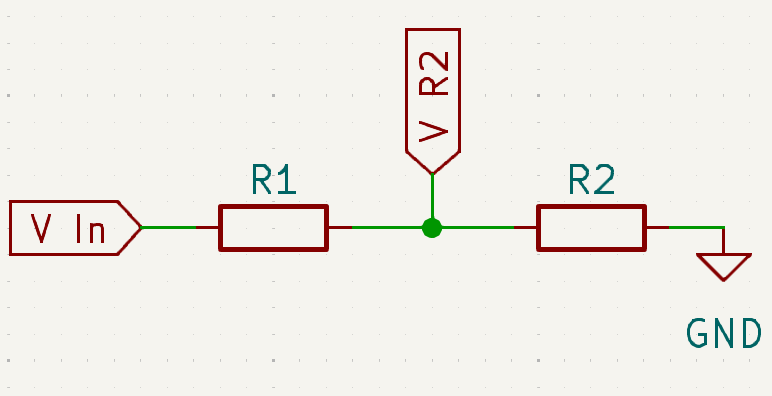
\includegraphics[width=0.6\textwidth]{figures/fig_voltage_divider.png}
    \caption{Simple voltage divider circuit used for resistance measurement.}
    \label{fig:voltage_divider}
\end{figure}

Equations~\ref{eqn:voltage_divider} and~\ref{eqn:resistance_divider} are used to calculate the resistance from the voltage divider equation.
\begin{equation}\label{eqn:voltage_divider}
    V_{R2} = V_{In} \times \frac{R_2}{R_1 + R_2}
\end{equation}
\begin{equation}\label{eqn:resistance_divider}
    R_2 = \frac{R_1 \times V_{R2}}{V_{In}-V_{R2}}
\end{equation}


\section{Circuit Design}\label{sec:circuit_design}
The probe circuit is the circuit which contains the resistor divider, was designed to be printed onto a \gls{pcb}.
This design was influenced by Reference~\cite{cam_clark}, where a similar device was designed for salinity measurements in ice columns.
A \gls{pcb} was chosen for this circuit as the researcher had significant experience with \gls{pcb} design, and the manufacturing process offered higher precision than hand soldering, and is relatively cost-effective.
Significant improvements and modifications were made to the resistor divider circuit, to allow for a wider range of testing.

For input power, a \gls{dac} was used to drive the circuit. This allowed to the input voltage to be varied between $0 V$ and the reference voltage, which was chosen to be $5V$.
This allowed for a range of voltages to be applied, which allowed for the measurement of the water's voltage-resistance relationship, and the creation of \gls{ac} signals.
A function generator was considered for generating the \gls{ac} signal, as it would allow for signals of a wider frequency and and high precision, however the price could not be accommodated by the budget.
The choice of \gls{dac}, and all following components, was first influenced by availability on JLCPCB, the \gls{pcb} manufacturing house.
The MCP4725 was chosen for its high resolution of 12-bits, offering a digital range of 0-4095, fast update time of $6{\mu}s$, and interface speed of 3.4MHz.
These features allow for both \gls{dc} and \gls{ac} signal analysis.

An op-amp with unity gain was the connected to the output of the \gls{dac}.
This is because \gls{dac}s have limited output drive capabilities, and the op-amp would allow for heavier loads to be driven.
Additionally the op-amp offers improved output stability, introduces impedance isolation, which protects the \gls{dac} from load variations and feedback effects, and allows for better sine wave quality.

As mentioned in Section~\ref{sec:res_mes}, for the resistor divider circuit, the electrodes would serve as $R_2$ and a known resistor as $R_1$.
Three alternative values of $R_1$ were chosen, to accommodate for any circuit errors.
These could be switched between using the TS3A4751 multiplexer \gls{ic}.
This switching multiplexer was chosen, for its low on-state resistance of $0.9\Omega$, and fast switching speed of $4-5ns$~\cite{cam_clark}.

The $R_1$ resistor values were chosen to be $100\Omega$, $1K\Omega$ and $10K\Omega$.
These values would be used when the resistance between the probes was $1-10\Omega$, $10-100\Omega$, and $100-1K\Omega$ respectively.
Each \gls{ic} contained 4 switches.

For measuring the output resistor, the voltage over it was directed into a multiplying op-amp with a gain of 11.
This increases the resolution for the \gls{adc} readings, as low voltages may be hard to differentiate between when converted to digital data. 

This configuration would allow for a minimum resolution of $11\%$ of $V_{DAC}$ and maximum of $100\%$ of $V_{DAC}$, for the voltage measurement by the \gls{adc}, as shown in Equations~\ref{eqn:dac_11} and~\ref{eqn:dac_100}~\cite{cam_clark}.
Equations~\ref{eqn:dac_11} and~\ref{eqn:dac_100} show for the expected resistance of $7.55\Omega$ falling into the $1-10\Omega$ range.
However, if the resistance falls into the $10-100\Omega$, or $100-1K\Omega$, the respective $R_1$ resistors would be used and the maximum and minimum \gls{dac} resolutions would be the same.

\begin{equation}\label{eqn:dac_11}
    \frac{1\Omega}{1\Omega + 100\Omega}\times V_{DAC} \times 11 = 11\% V_{DAC}
\end{equation}

\begin{equation}\label{eqn:dac_100}
    \frac{10\Omega}{10\Omega + 100\Omega}\times V_{DAC} \times 11 = 100\% V_{DAC}
\end{equation}

The accuracy of the $R_1$ resistor is integral to achieving an accurate $R_2$ measurement.
The resistors available on JLCPCB had an accuracy of $\pm{1}\%$.
To increase the accuracy 3 equal resistors were put in parallel. This decreases the uncertainty of the total equivalent resistance~\cite{cam_clark}.
This is shown in Equations~\ref{eqn:parallel_r} to~\ref{eqn:resistance_uncertainty}.

\begin{equation}\label{eqn:parallel_r}
    R_{T} = {\left[{\sum_{i=1}^{n}{\frac{1}{R_n}}}\right]}^{-1}
\end{equation}

If all the Resistors are equal this simplifies to: 

\begin{equation}\label{eqn:parallel_r_equal}
    R_{T} = ({\frac{n}{R}})^{-1} = \frac{1}{n} \times R
\end{equation}

To propagate uncertainty the standard equation for combined uncertainty can be used: \\
\hspace*{2em}~If a quantity $y$ depends on several independent variables $x_1, x_2, \ldots, x_n$: \\
\hspace*{2em}~$y=f(x_1, x_2, ..., x_n)$ \\
\hspace*{2em}~and each $x_i$ has a standard uncertainty $u(x_i)$ then the combined standard uncertainty \\
\hspace*{2em}~of $y$, denoted $u_c(y)$, is:

\begin{equation}\label{eqn:standard_uncertainty}
    \delta_y=\sqrt{\sum_{i=1}^{n}{\left({{\frac{\partial{f}}{\partial{x_i}}}{\delta_{x_i}}}\right)}^2}
\end{equation}

For Resistance this can be shown as:

\begin{equation}\label{eqn:resistance_uncertainty}
    \delta_{R_T}=\sqrt{\sum_{i=1}^{n}{\left({{\frac{\partial{R_{T}}}{\partial{R}}}{\delta_{R}}}\right)}^2} = \sqrt{{\left({{\frac{1}{n}}\delta_R}\right)}^2} = \frac{1}{n}\delta_R
\end{equation}

Using the above equations, with resistors with an individual uncertainty of $\pm1\%$, three resistors in parallel have a combined uncertainty of $\pm0.33\%$
To created the intended $R_1$ resistances of $100\Omega$, $1K\Omega$ and $10K\Omega$, the three parallel resistors were chosen to use values of $300\Omega$, $3K\Omega$ and $30K\Omega$ respectively.

A second switch circuit was then used to configure the $R_2$ resistor.
With there being two electrodes, the switching circuit allowed for the user to choose which would be the anode and the cathode.
The switch also included a calibration resistor of $5\Omega$, which would allow for the calculation of the gain of the \gls{adc} when measuring.
This calibration resistor was also created using a parallel resistor configuration, where four $20\Omega$ resistors were connected in parallel to give the require resistance at an uncertainty of $\pm0.25\%$.

A simplified circuit diagram showing the resistance measuring circuit is shown in Figure~\ref{fig:resistance_circuit}.

\begin{figure}[H]\label{fig:resistance_circuit}
    \centering
    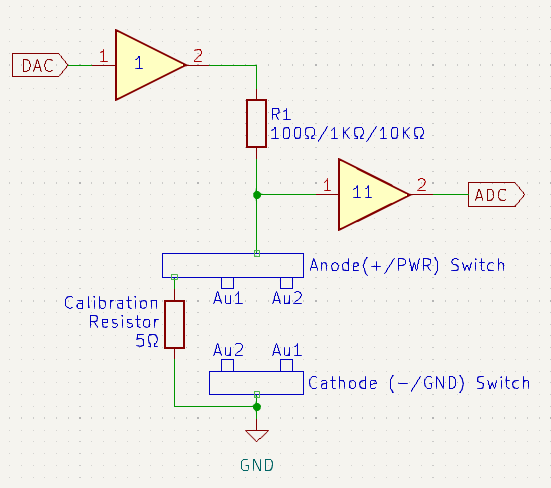
\includegraphics[width=0.75\textwidth]{figures/fig_resistance_circuit.png}
    \caption{Simple circuit diagram of the resistance measuring circuit.}
    \textit{Note: Au1 Denotes Gold Electrode 1, and Au2 Gold electrode 2.}
    \label{fig:resistance_circuit}
\end{figure}

A third switch was added to allow for the configuration of the fringe guard, allowing the fringe guard paired with an electrode to share the same voltage configuration, i.e.~when an electrode acted as the anode its fringe guard would also act as an anode, and vice versa.
The voltage of $R_1$ was directed through a unity gain buffer op-amp, and then connected on its output to the fringe guard, allowing for the same voltage over the electrodes to be over the fringe guards without affecting the measurement of the electrode voltage.

Four points on the resistance circuit were routed to separate \gls{adc}s, and a test point added to allow for the comparison between the voltage measured by the \gls{adc} and by a multimeter.
These points were at the \gls{dac} output before the unity gain buffer op-amp, after the unity gain buffer op amp, before the 11x multiplying op-amp and after the 11x multiplying op-amp.
A separate capacitor was connected across each of these points and ground to stabilise the \gls{adc} readings and remove noise.
These capacitors were connected via switches, to allow them to be disconnected when an \gls{ac} signal needed to be measured.
Two additional test points were added to measure the rail voltages from the voltage regulators.

In addition to the resistance measuring circuitry, a waterproof pressure and temperature sensor was included, as these values are needed for calculating salinity.
The MS583702BA01-50 was chosen for its low price and availability on JLCPCB.
This sensor only allowed for up to 2 Bar pressure measurements, which was enough for this prototype, but would not satisfy the real-world requirements of the salinity probe.
Lastly, an RS-485 \gls{ic} was included for inter board communication.

A ESP-32 S2-Mini-2 was chosen for the microcontroller, as it was the most cost effective ESP32 based microcontroller.
It offered an FPU, allowing for the complex salinity calculations to be done, did not require a \gls{uart} bridge as it has built-in USB OTG support, allowing it to connect directly to a computer for easy programming, which was done via a USB-Micro port, and offered 13-bit \gls{adc}s, allowing for a good voltage measurement resolution.
Additionally the wireless capabilities allowed for easy debugging, through a web interface, as the researcher's computer only had one USB port.
The researcher also had significant experience with this microcontroller.

A controller \gls{pcb} was designed alongside the probe \gls{pcb}.
This controller was designed to communicate with the probe while it was submerged, sending it instructions and receiving results.
It allowed for the measurements to be recorded in a $.txt$ file on a micro-SD card, and displayed on a $16\times2$ LCD screen.
The \gls{pcb} for this controller was minimal, and relied on external breakout circuit boards.
This was due to budget constraints, and did not affect the effectiveness of the controller.
Only the voltage regulation circuitry, and inter-board communication (RS-485) circuitry were included in the production.
Headers were included on the controller \gls{pcb} to allow an ESP-Wroom-32 Devkit module to be mounted to it.
Additional headers were included to allow the breakout boards for the LCD display and SD card reader to connect to the ESP32. 

For the inter-board connection the RS-485 communication protocol was chosen.
The ESP32 microcontrollers do support wireless communication through bluetooth and Wi-Fi.
However, wireless communication, especially electro-magnetic waves suffer interference~\cite{waves_in_water}.
A wired connection medium, the RS-485 protocol was chosen. 
Compared to most other communication protocols which typically support distances no longer than $\pm50m$, RS-485 supports up to 1200m, and has good underwater stability.
The \gls{ic} only requires simple $I^2C$ and is relatively cheap.
RS-485 usually uses a pair of twisted cables, which strengthens the electromagnetic magnetic interference rejection and reduces signal degradation.
However, due to availability, simple 4-core communication was used, where the additional two cores were used to transmit power between the \gls{pcb}s.

\section{Assembly and Programming}
\subsection{PCB and Circuit Assembly}
The Probe, Controller and electrode circuitry \gls{pcb}s were designed using KiCAD software, and manufactured by JLCPCB. The KiCAD design files for these can be found in the GitHub repository linked in Appendix~\ref{app:c_github}.

The probe \gls{pcb} had dimensions of $50\times50$mm and was fabricated onto a 4-layer \gls{pcb}.
This was chosen as the probe would need to fit in the ice hole with a diameter of 100mm, and JLCPCB offers a discounted rate on 4-layer \gls{pcb}s if the dimensions are $50\times50$mm or less. 
This size also made debugging easier.
In addition to the components required for transmission and measurement, test points with headers were added for easy debugging, and an indicator \gls{led}, to indicate power.
The probe is shown in Figure~\ref{fig:probe_pcb}.

%space


The controller was relatively simple, and only require a 2-layer \gls{pcb}, with dimensions of $70\times55mm$.
This size and layer count fell into the same discounted bracket as the probe \gls{pcb}.
The external micro-SD card reader was connected to the \gls{pcb} through a breadboard.
The chosen ESP32-Wroom Devkit module when designing the \gls{pcb} was not the same one the researcher had access to when assembling the controller, and differed in size.
To accommodate for this the available ESP32-Wroom module was also placed on the breadboard and was connected to the \gls{pcb} via jumper cables.
Additionally the 16x2 LCD display was not used because of this.
The complete Controller \gls{pcb} and additional circuitry can be seen in Figure~\ref{fig:controller_pcb}.

\begin{figure}[H]
    \begin{minipage}{0.5\textwidth}
        \centering
        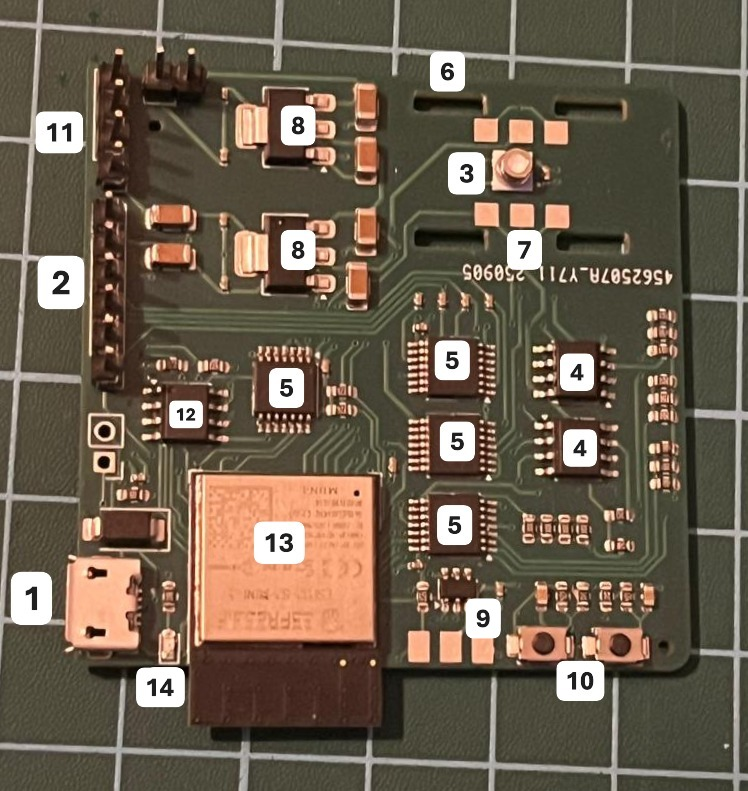
\includegraphics[width=0.8\textwidth]{Figures/probe_pcb.jpg}
    \end{minipage}
    \begin{minipage}{0.5\textwidth}
        \centering
        \begin{tabular}{cl} \hline
            1 & USB-Micro Port \\ \hline
            2 & Test Points \\ \hline
            3 & Pressure Sensor \\ \hline
            4 & Op-Amps \\ \hline
            5 & Switch \gls{ic}s \\ \hline
            6 & Gold Electrode Mounts \\ \hline
            7 & Gold Electrode Solder Pads \\ \hline
            8 & Voltage Regulators \\ \hline
            9 & \gls{dac} \\ \hline
            10 & Boot and Enable Buttons\\ \hline
            11 & RS-485 Port \\ \hline
            12 & RS-485 \gls{ic} \\ \hline
            13 & ESP32 Microcontroller \\ \hline
            14 & Power Indicator \gls{led} \\ \hline
        \end{tabular}
    \end{minipage}
    \caption{The probe PCB}
    \label{fig:probe_pcb} %chktex 24
\end{figure}

\begin{figure}[H]
    \begin{minipage}{0.5\textwidth}
        \centering
        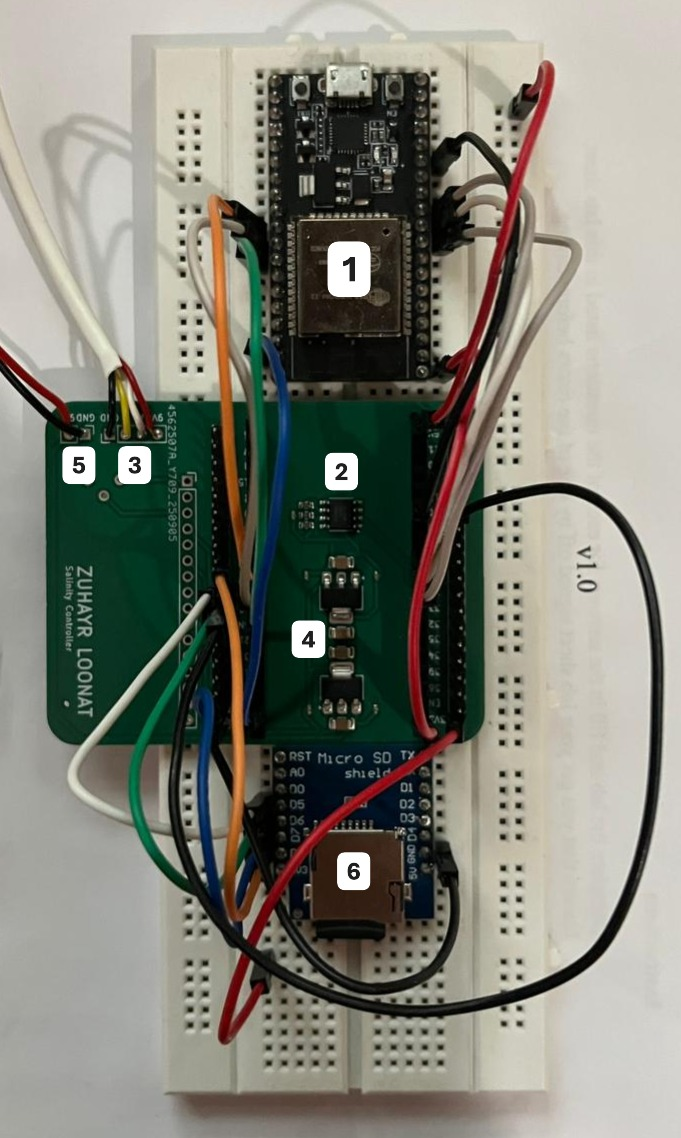
\includegraphics[width=0.8\textwidth]{Figures/controller_circuit.jpg}
    \end{minipage}
    \begin{minipage}{0.5\textwidth}
        \centering
        \begin{tabular}{cl} \hline
            1 & ESP32-Wroom-Devkit \\ \hline
            2 & RS-485 IC \\ \hline
            3 & RS-485 Port \\ \hline
            4 & Voltage Regulators \\ \hline
            5 & Input Power \\ \hline
            6 & Micro-SD Card Reader \\ \hline
        \end{tabular}
    \end{minipage}
    \caption{Controller PCB and Additional Circuitry}
    \label{fig:controller_pcb} %chktex 24
\end{figure}

\hfill \break

The two \gls{pcb}s were connected via 4-core communication cable, with pins for RS-485 Tx and Rx, Ground and 9V Power.
Additionally, 6 core wire was connected to the probe \gls{pcb} along the 6 test points, to allow for easy debugging when submerged.
Both PCBs were powered by an input voltage of 9V which was stepped down appropriately, using voltage regulator \gls{ic}s, for a stable power input.

The electrode manufacturing was simple, as it consisted of the gold plated solder pads, as mentioned in Section~\ref{sec:electrode_design}.
No additional modifications had to be made to the electrode \gls{pcb}s, and they were hand soldered to the corresponding solder pads on the probe \gls{pcb}.

\subsection{Waterproofing}\label{sec:waterproofing}
Since the probe \gls{pcb} would need to be submerged in water, it will would need to waterproofed.
A multitude of methods were considered including conformal coating, a 3D-printed waterproof enclosure, and resin casting.
Conformal coating is a thin protective layer applied to shield circuitry and \gls{pcb}s from moisture and extreme temperature, and usually comes in a spary can.
It is relatively cheap but has a low pressure resistance, and offers low physical protection.
A 3D-printed enclosure was considered too complex, ultimately leaving a resin cast as the chosen method.
This method offers good physical protection and is considered the most reliable.

The RE33/HE33 resin from AMT Composites was chosen for the \gls{pcb} to be cast in, as it is specifically designed for the encapsulation of electrical components.
The cast was made using acrylic sheeting, which were chosen because they do not stick to the resin.
The sheets were cut using a hack saw and joined using waterproof superglue.

The electrodes were spaced using two pieces of acrylic measured to 10mm (i.e.~the electrode separation distance).
A plastic straw was used to isolate the pressure sensor as the diameter of the stray matched the pressure sensor perfectly.
This ensured that the sensor could measure the pressure of the water accurately.
The required cables were soldered to the \gls{pcb} before pouring the resin.
A fully encapsulated probe \gls{pcb} can be seen in Figure~\ref{fig:encapsulated_probe}.

\begin{figure}[H]
    \begin{minipage}{0.5\textwidth}
        \centering
        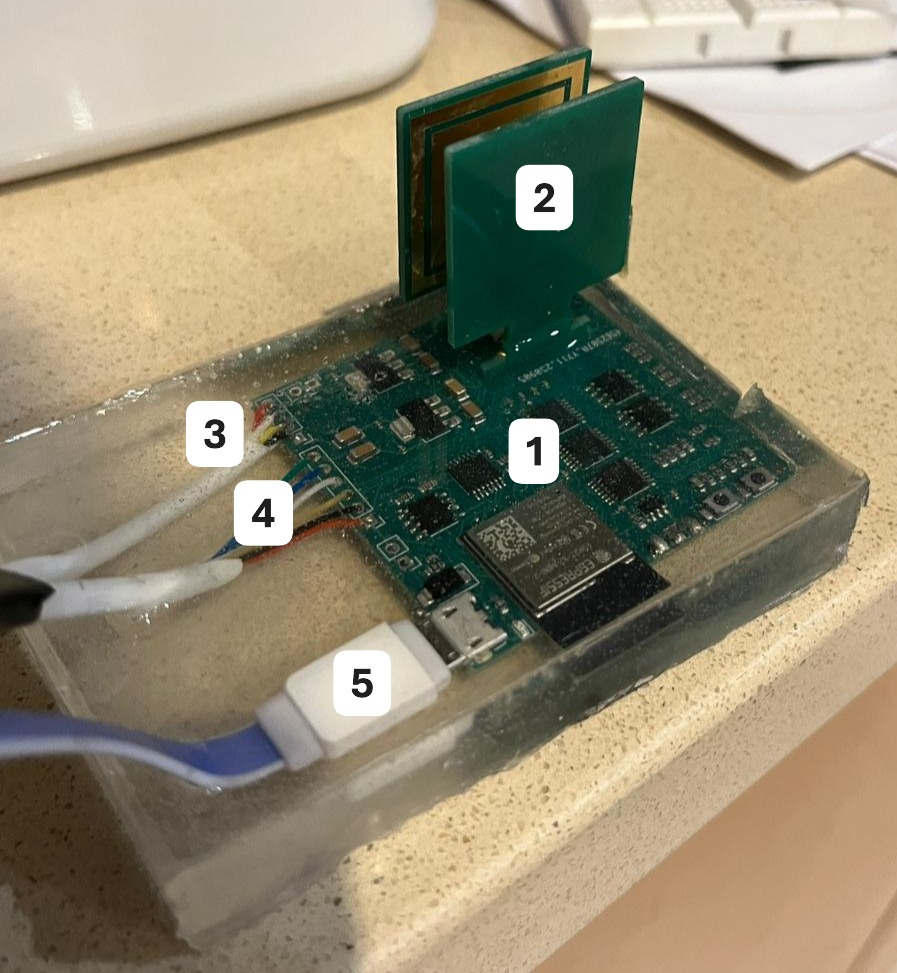
\includegraphics[width=0.8\textwidth]{Figures/encapsulated_probe.jpg}
    \end{minipage}
    \begin{minipage}{0.5\textwidth}
        \centering
        \begin{tabular}{cl} \hline
            1 & Probe Board \\ \hline
            2 & Gold Electrodes \\ \hline
            3 & RS-485 and Power Cable \\ \hline
            4 & Test Point Cable \\ \hline
            5 & Programming Cable \\ \hline
        \end{tabular}
    \end{minipage}
    \caption{Encapsulated Probe}
    \label{fig:encapsulated_probe} %chktex 24
\end{figure}

\subsection{Microcontroller Programming}\label{sec:uc_program}
The controller was programmed to send commands to the probe via RS-485, and the probe to follow the command and return the data back to the controller.
These commands would first be sent by a computer to the serial monitor on the controller board, and then would be sent from the controller to the probe.
Multiple measurement modes were programmed into the probe board and they were triggered with specific commands.
A separate C++ header file, with functions for the salinity calculation equations, mentioned in Section~\ref{sec:salinity_compensation}, was created for ease of coding and and reusability.

The voltage measurements were done using the ESP32's built in \gls{adc}s, which used a reference voltage of $3.3V$.
To account for measurement inaccuracies caused by the \gls{dac}, \gls{adc} or op-amp, the calibration resistor was used to find a calibration factor, which will be denoted by $C_F$.
This factor was calculated by connecting the calibration resistor ($R_2$) to a chosen $R_1$ resistor, and measuring the voltage drop over it.
This value would then be compared to the expected voltage drop, calculated mathematically.
The expected voltage is divided by the measured voltage to give the calibration factor $C_F$.
Readings from the \gls{adc} would then be multiplied by this calibration factor, removing any inaccuracies.
The calculation of the calibration factor is shown in Equations~\ref{eqn:caibration_equation1} to~\ref{eqn:caibration_equation4}.

\begin{gather}
    \text{Given calibration resistor }R_{C} = 5\Omega \label{eqn:caibration_equation1} \\
    \text{Expected }V_{C} = 11\times V_{IN}\times\frac{R_C}{R_C+R_1} \\
    \text{Measured }V_{C} = \frac{\text{ADC Reading}}{\text{ADC Resolution}} \times V_{Ref} \\
    \text{Calibration Factor }C_F = \frac{\text{Expected }V_C}{\text{Measured }V_C} \label{eqn:caibration_equation4}
\end{gather}

Measurement modes were created for calibration testing, \gls{dc} analysis and \gls{ac} analysis.
For all these modes voltage measurements using the \gls{adc}s were taken before the unity gain buffer op-amp, after the unity gain buffer op amp, before the 11x multiplying op-amp and after the 11x multiplying op-amp.
Additionally temperature and pressure readings were taken for all modes, to allow for corrections.
All salinity calculations were calculated using the PSS-78 equations mentioned in Section~\ref{sec:salinity_compensation}.

\subsubsection{Calibration Test}
The calibration test function was designed to measure the inaccuracies of the \gls{adc}s, \gls{dac} and op-amp, and to return a calibration factor based on these inaccuracies.
It used Equations~\ref{eqn:caibration_equation1} to~\ref{eqn:caibration_equation4} to achieve this.

\subsubsection{DC Voltage Sweep}
This procedure was designed to take voltage measurements over the probes through a range of voltages, were the function allowed for the maximum voltage, and chosen $R_1$ resistor, to inputted.
The \gls{dac} would output a voltage, the calibration resistor would be measured to calculate the calibration factors for each \gls{adc} and then the electrode voltages would be measured bi-directionally ($Au_1$ as +, $Au_2$ as negative, and vice versa).
This would be done for the full specified range of voltages in increments of $0.1V$.

A resistance would then be calculated for the corresponding voltage, and this would be used to calculate the conductivity.
The conductivities and resistances for each voltage step would be returned as well as the temperature and pressure values.
The average conductivity is also returned. This is shown in Figure~\ref{fig:dcsweep}.

\subsubsection{DC Single Voltage}
This function was designed to take a single voltage reading.
Similar to the \gls{dc} voltage sweep, this first measures over the calibration resistor, to find the calibration factor, and then takes bi-directional measurements over the electrodes.
the voltage is then used to calculate the conductivity, which was returned with the temperature and pressure values.
This is shown in figure~\ref{fig:dcpoint}

Essentially, the voltage sweep performed the single voltage test through a range of voltages.

\begin{figure}[H]
    \centering
    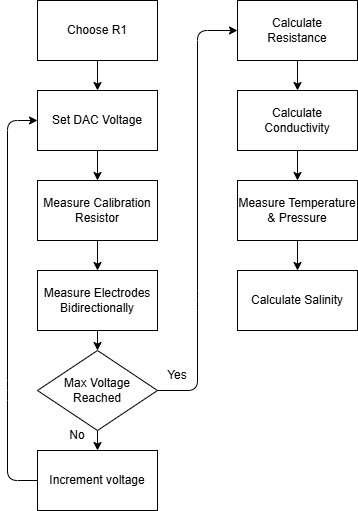
\includegraphics[width=0.4\textwidth]{figures/dcsweep.png}
    \caption{DC Sweep Function}
    \label{fig:dcsweep}
\end{figure}

\begin{figure}[H]
    \centering
    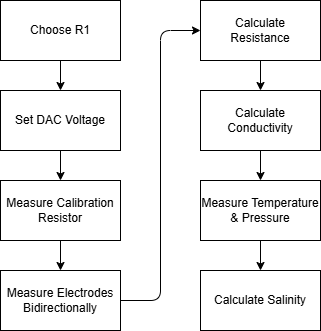
\includegraphics[width=0.4\textwidth]{figures/dcpoint.png}
    \caption{DC Single Voltage Function}
    \label{fig:dcpoint}
\end{figure}

The \gls{dc} procedures were first to be done on the standard solution of 35 \gls{psu} at $15^{\circ}C$, mentioned in Section~\ref{sec:salinity_theory}.
This allowed for the conductivity of the standard solution to be calculated, as the calculation of salinity relies on the ratio between the salinity of the standard solution and the sample solution.

\subsubsection{AC Wave Generator}
For \gls{eis}, \gls{ac} signals are used. This function allowed for a frequency and amplitude to be inputted.
It would then output a sinusoidal waveform using the \gls{dac}, and the output over the electrodes would be measured.
This allowed for the values of the input and output waveform to be returned.
For the duration of this function, the stabilising capacitors connected to the \gls{adc}s, mentioned in Section~\ref{sec:circuit_design} were disconnected, as they would interfere with the \gls{ac} signal.

The values for the input and output waves were exported to a $.csv$ file and then processed in MATLAB and python.

\subsubsection{Inter-Board Communication}
As mentioned previously, the controller board was programmed to send instructions to the probe, and receive the readings for those functions, from the probe.
Half-Duplex RS-485 was effectively used as only one board could communicate at a time.
The probe board would be set by default to receive mode, and controller to transmit mode.
The controller would send an instruction to the probe, and would then change to receive mode, awaiting the readings from the probe.
Once the probe received the instruction it would change to transmit mode, allowing it to send the readings.
Once the readings were sent, the probe would return to receive mode, and upon receiving the readings the controller would return to transmit mode.
The controller instructions were typed in manually via the controller's serial monitor.
Upon receiving the readings, the controller would display them in the serial monitor and print them to the $.txt$ file on the micro-SD card.
This process is shown in Figure~\ref{fig:comms}.

\begin{figure}[H]
    \centering
    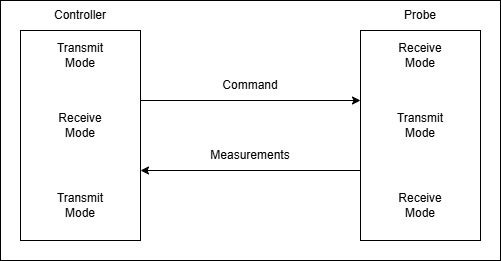
\includegraphics[width=0.7\textwidth]{figures/comms.png}
    \caption{Communication Protocol}
    \label{fig:comms}
\end{figure}

\subsection{Machine Learning Programming and AC Analysis}\label{sec:ml_for_eis}

For salinity prediction through \gls{eis}, impedance measurements over a range of input frequencies and amplitudes would need to be taken.
This would allow the machine learning to be formatted as a regression task, where the input features consist of:
\begin{itemize}
    \item AC excitation frequency $(f)$
    \item AC excitation amplitude $(A)$
    \item Measured impedance magnitude $|Z|$
    \item Measured phase angle $(\phi)$
\end{itemize}

For linear systems AC excitation amplitude is not necessary, however, for non-linear systems, such as this, it needs to be included, as the measured impedance may be affected by the excitation amplitude.
The output is the predicted salinity value. During the training the model learns the mapping function (function is denoted with $m$ instead of $f$ as $f$ is used to represent frequency):
\begin{equation}
    \text{Salinity}= m(f,A,|Z|,\phi)
\end{equation}

Multiple input frequency-amplitude combinations can be used as input features, enabling the model to leverage information across the entire impedance spectrum for improved salinity accuracy~\cite{wang_deep_2024}.

For \gls{eis} salinity measurements, neural networks would theoretically be the superior choice~\cite{doonyapisut_analysis_2023}.
This is due to their ability to model highly complex, non-linear relationships which are inherent in electro-chemical systems~\cite{chen_intelligent_2025}.
They have the ability to automatically learn feature interactions, without manual feature engineering and their ability to learn hierarchical representations makes them especially suited for \gls{eis} data~\cite{doonyapisut_analysis_2023}.
However, given the constraint of a small sample size, random forest is the more practical and effective choice for this application.
Random forests require significantly less training data to achieve reliable performance, often working well with just dozens to hundreds of samples rather than the thousands needed for neural networks.
With limited data, neural networks are highly prone to over-fitting, essentially memorising the training examples rather than learning generalisable patterns, which would result in poor performance on new salinity measurements~\cite{alwosheel_is_2018}.
Random forests mitigate this through their ensemble approach (using multiple smaller models), which reduces variance and improves robustness even with small data sets. 
Additionally they require minimal parameter tuning and work reasonably well `out of the box', whereas neural networks require extensive architecture design, learning rate optimisation, and regularisation techniques that become nearly impossible to properly tune without sufficient validation data~\cite{alwosheel_is_2018}.

Due to these factors random forest was chosen.
The programming for this model was done in python via a Jupyter Notebook, as this is widely used in the industry.
First, to test the random forest model, a Resistor-Capacitor dataset was used,
This allowed for the evaluation of the accuracy of the model.
It used an input frequency and amplitude and output impedance magnitude and phase, mapped to a dielectric permittivity (the other parameters for capacitance were the same for all capacitor values), to predict permittivity of the capacitor, based on the inputs.
Once the Resistor-Capacitor model was tested, the model was updated to support the \gls{eis} parameters for salinity.

To create the \gls{eis} dataset for the random forest model, measurements of signals of varying frequency and amplitude, in solutions of varying salinity would be taken.
It was planned to use 10 solutions of varying salinity, with frequencies 1-100Hz in increments of 20Hz, since the MCP4725 \gls{dac} outputted these reliably, and amplitude 0-1V in increments of 0.2V.
This would give a total dataset of 360 data points, enough to train the random forest on.